\documentclass{article}
\usepackage{graphicx}% Required for inserting images
\usepackage{caption}
\graphicspath{{images/}}

\title{Mi crush de la secu}
\author{Nicolás Bustos}
\date{Septiembre 2026}

\begin{document}

\maketitle

\section{Primera parte: casi algo}
Allá por el lejano 2016, cuando yo cursaba el segundo año de secundaria, entré a una nueva escuela y conocí a la morrita más \textbf{preciosa} que mis ojos habían visto: 
\begin{itemize}
  \item Alta
  \item Güerita
  \item Inteligente
  \item Graciosa
  \item Guapa
  \item Con pedos psicológicos
\end{itemize}
Ah, no, eso último no iba.
\\Era el combo completo, pa' acabar pronto.
\\
\\¿Y el problema? pues que ella \textit{ya tenía novio ca'wn.} Igual yo hice mi intento, y entre que sí y que no, \textbf{me aceptó una salida.}
\\La pasamos bien, nos reímos, hablamos de libros, de series, de gustos musicales, incluso compartimos audífonos para escuchar música por un buen rato (audífonos de cable, obvio), paseamos en el parque, todo estuvo increíble y para el final del día, sin necesidad de decirlo, ya ambos sabíamos que el sentimiento era mutuo.
\\
\\Ahora el dilema era saber qué hacer con eso. 
\\
\\Después de mucho pensarle, llegué a la conclusión de que si realmente ella también sentía algo por mí, dejaría a su novio. Entonces yo aprovecharía ese momento y le preguntaría si quería ser mi novia y ella saltaría a mis brazos y me diría que sí y seríamos felices para siempre.
\\
\\Así de ingenuo yo, pero tenía 14 años, no se me pongan tan exigentes.
\\
\\Evidentemente, ese momento no llegó, y mientras pasaba el año escolar, y los días se imprimían con la tinta del bolígrafo sobre las hojas de nuestras libretas, y el clima se tornaba caluroso anunciando la llegada del verano (ay sí, el poético), el tiempo se nos escapó de las manos, y me obligó a soportar la larga espera del periodo vacacional para volver a verla.
\section{Segunda parte: el regreso a clases}
Nervioso, emocionado y expectante, imaginando que ese periodo de ausencia podría haber distanciado a \textit{Ximena} de su anterior novio, entré al nuevo salón de clases. Busqué su rostro por entre muchos conocidos y alguno que otro nuevo.
\\No estaba.
\\Desesperado, al no encontrarla, comencé a observar las mochilas en las bancas vacías, a ver si por casualidad lograba reconocer la suya, y elegir lugar a un lado.
\\
\\Nada.
\\
\\El reloj avanzaba más lento de lo que jamás había experimentado, mientras se volvía más remota la posibilidad de que, a último minuto, ella entrara por la puerta.
\\
\\Llegó el profesor.
\\
\\Acomodó su portafolio el escritorio.
\\
\\Sacó los gises, colocó el borrador en el pizarrón, miró a la bulliciosa masa de adolescentes con cierto desprecio.
\\
\\Y Ximena no había llegado.
\\
\\A punto de que el timbre que anuncia las 7 terminara con mis últimas esperanzas de volver a verla, llegó corriendo, sonrojada por el esfuerzo, entró al salón, y sin siquiera verme, se sentó al lado mío. 
\\
\begin{figure}[h]
    \centering
    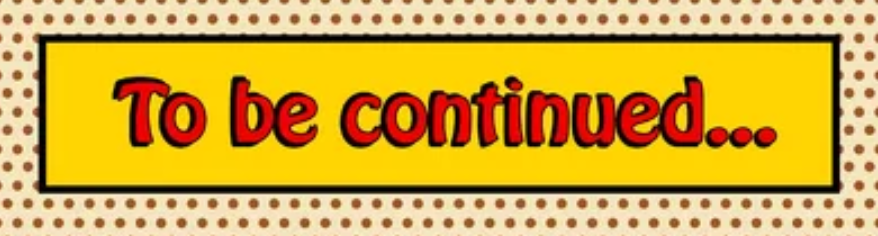
\includegraphics[width=0.5\linewidth]{Continuará.png}
    \captionsetup{labelformat=empty}
    \caption{\small \textit{Disclaimer: Algunos de los hechos plasmados en el texto han sido exagerados con fines de entretenimiento al lector.}}
    \label{fig:placeholder}
\end{figure}
\\

\end{document}
